\subsection{2016 Free-Response Questions}
Questions 1 and 2 part of the same section area are allotted 30 minutes from completion with the aid of a graphing calculator.
Questions 3 through 6 are part of the same section and area allotted 1 hour from completion without the aid of a graphing calculator.

\begin{table}[H]
	\begin{center}
		\begin{tabular}{|c||c|c|c|c|c|}
			\hline
			$t$ (hours) & 0 & 1 & 3 & 6 & 8 \\
			\hline
			$R(t)$ (liters / hour) & 1340 & 1190 & 950 & 740 & 700 \\
			\hline
		\end{tabular}
	\end{center}
\end{table}

\begin{enumerate}
	\item Water is pumped into a tank at a rate modeled by $W(t)=2000e^{-t^2/20}$ liters per hour for $0 \leq t \leq 8$, where $t$ is measured in hours.
	Water is removed from the tank at a rate modeled by $R(t)$ liters per hour, where $R$ is differentiable and decreasing on $0 \leq t \leq 8$.
	Selected values of $R(t)$ are shown in the table above.
	At time $t=0$, there are 50000 liters of water in the tank.
	\begin{enumerate}
		\item Estimate $R^\prime(2)$.
		Show the work that leads to your answer.
		Indicate units of measure.
		\item Use a left Riemann sum with the four subintervals indicated by the table to estimate the total amount of water removed from the tank during the 8 hours.
		Is this an over estimate or underestimate of the total amount of water removed?
		Give a reason for your answer.
		\item Use your answer from part (b) to find an estimate for the total amount of water in the tank, to the nearest liters, at the end of the 8 hours.
		\item For $0 \leq t \leq 8$, is there a time $t$ when the rate at which the water is pumped into the tank is the same rate as the rate at which water is removed from the tank?
		Explain why or why not.
	\end{enumerate}

	\begin{figure}[H]
		\label{2016_2}
		\centering
		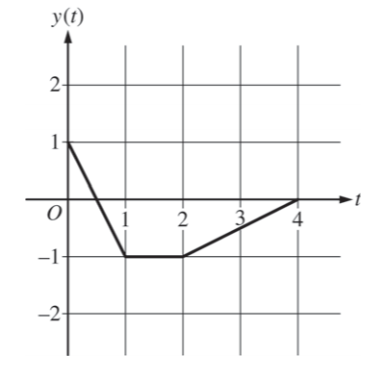
\includegraphics{./additional_materials/2016_2.png}
		\caption{\hyperref{https://secure-media.collegeboard.org/digitalServices/pdf/ap/ap16\_frq\_calculus\_bc.pdf}{}{}{AP Calculus BC 2016 Exam Free-Response Question 2}}
	\end{figure}
	
	\item At time $t$, the position of a particle moving in the $xy$-plane is given by the parametric functions $(x(t),y(t))$, where $\dd{x}{t} = t^2 + \sin{(3t^2)}$.
		The graph of $y$ consisting of three line segments, is shown in the figure above.
		At $t=0$, the particle is at position $(5,1)$.
		\begin{enumerate}
			\item Find the position of the particle at $t=3$.
			\item Find the slope of the line tangent to the part of the particle at $t=3$.
			\item Find the speed of the particle at $t=3$.
			\item Find the total distance traveled by the particle from $t=0$ to $t=2$.
		\end{enumerate}
	
	\begin{figure}[H]
		\label{2016_3}
		\centering
		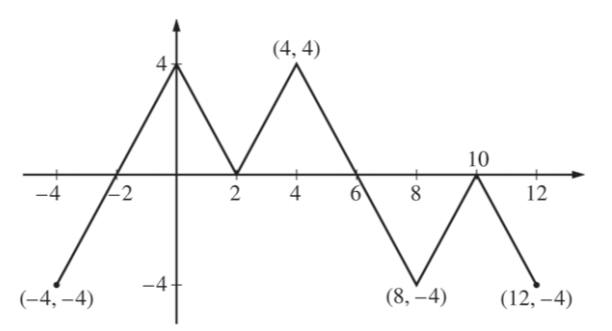
\includegraphics{./additional_materials/2016_3.png}
		\caption{\hyperref{https://secure-media.collegeboard.org/digitalServices/pdf/ap/ap16\_frq\_calculus\_bc.pdf}{}{}{AP Calculus BC 2016 Exam Free-Response Question 3, Graph of $f$}}
	\end{figure}
	
	\item The figure above shows the graph of the piecewise-linear function $f$.
		For $-4 \leq x \leq 12$, the function $g$ is defined by $g(x)=\int_{2}^{x}{f(t)\d{t}}$.
		\begin{enumerate}
			\item Does $g$ have a relative minimum, a relative maximum, or neither at $x=10$?
				Justify your answer.
			\item Does the graph of $g$ have a point of inflection at $x=4$?
				Justify your answer.
			\item Find the absolute minimum value and the absolute maximum value of $g$ on the interval $-4 \leq x \leq 12$.
				Justify your answers.
			\item For $-4 \leq x \leq 12$, find all intervals for which $g(x) \leq 0$.
		\end{enumerate}
	
	\item Consider the differential equation $\dd{y}{x} = x^2 - \frac{1}{2}y$.
		\begin{enumerate}
			\item Find $\dd{^2y}{x^2}$ in terms of $x$ and $y$.
			\item Let $y=f(x)$ be the particular solution to the given differential equation whose graph passes through the point $(-2,8)$.
				Does the graph of $f$ have a relative minimum, a relative maximum, or neither at the point $(-2,8)$?
				Justify your answer.
			\item Let $y=g(x)$ be the particular solution to the given differential equation with $g(-1)=2$.
				Find $\lim_{x\to -1}{\left(\frac{g(x)-2}{3(x+1)^2}\right)}$.
				Show the work that leads to your answer.
			\item Let $y=h(x)$ be the particular solution to the given differential equation with $h(0)=2$.
				Use Euler's method, starting at $x=0$ with two steps of equal size, to approximate $h(1)$.
		\end{enumerate}
	
	\begin{figure}[H]
		\label{2016_5}
		\centering
		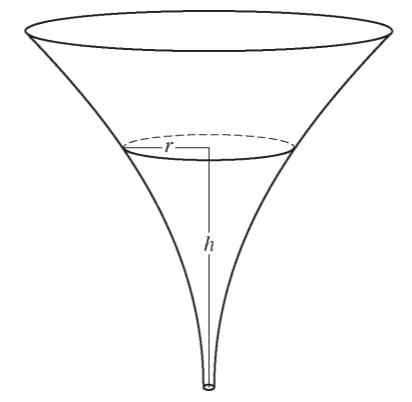
\includegraphics{./additional_materials/2016_5.png}
		\caption{\hyperref{https://secure-media.collegeboard.org/digitalServices/pdf/ap/ap16\_frq\_calculus\_bc.pdf}{}{}{AP Calculus BC 2016 Exam Free-Response Question 5}}
	\end{figure}
	
	\item The inside of a funnel of height 10 inches has circular cross sections, as shown in the figure above.
		At height $h$, the radius of the funnel is given by $r = \frac{1}{20}\left(3+h^2\right)$, where $0 \leq h \leq 10$.
		The units of $r$ and $h$ are inches.
		\begin{enumerate}
			\item Find the average value of the radius of the funnel.
			\item Find the volume of the funnel.
			\item The funnel contains liquid that is draining from the bottom.
				At the instant when the height of the liquid is $h=3$ inches, the radius of the surface of the liquid is decreasing at a rate of $\frac{1}{5}$ inch per second.
				At this instant, what is the rate of change of the height of the liquid with respect to time?
		\end{enumerate}
	
	\item The function $f$ has a Taylor series about $x=1$ that converges to $f(x)$ for all $x$ in the interval of convergence.
		It is known that $f(1)=1$, $f^\prime(1)=-\frac{1}{2}$, and the $n$th derivative of $f$ at $x=1$ is given by $f^{(n)}(1) = (-1)^{n}\frac{(n-1)!}{2^n}$ for $n \geq 2$.
		\begin{enumerate}
			\item Write the first four nonzero terms and the general term of the Taylor series for $f$ about $x=1$.
			\item The Taylor series for $f$ about $x=1$ has a radius of convergence of 2.
				Find the interval of convergence.
				Show the work that leads to your answer.
			\item The Taylor series for $f$ about $x=1$ can be used to represent $f(1.2)$ as an alternating series.
				Use the first three non-zero terms of the alternating series to approximate $f(1.2)$.
			\item Show that the approximation found in part (c) is within 0.001 of the exact value of $f(1.2)$.
		\end{enumerate}
\end{enumerate}